%-----------------------------------------------------------------------------------------------------------------------------------------------%
%	The MIT License (MIT)
%
%	Copyright (c) 2019 Jan Küster
%
%	Permission is hereby granted, free of charge, to any person obtaining a copy
%	of this software and associated documentation files (the "Software"), to deal
%	in the Software without restriction, including without limitation the rights
%	to use, copy, modify, merge, publish, distribute, sublicense, and/or sell
%	copies of the Software, and to permit persons to whom the Software is
%	furnished to do so, subject to the following conditions:
%	
%	THE SOFTWARE IS PROVIDED "AS IS", WITHOUT WARRANTY OF ANY KIND, EXPRESS OR
%	IMPLIED, INCLUDING BUT NOT LIMITED TO THE WARRANTIES OF MERCHANTABILITY,
%	FITNESS FOR A PARTICULAR PURPOSE AND NONINFRINGEMENT. IN NO EVENT SHALL THE
%	AUTHORS OR COPYRIGHT HOLDERS BE LIABLE FOR ANY CLAIM, DAMAGES OR OTHER
%	LIABILITY, WHETHER IN AN ACTION OF CONTRACT, TORT OR OTHERWISE, ARISING FROM,
%	OUT OF OR IN CONNECTION WITH THE SOFTWARE OR THE USE OR OTHER DEALINGS IN
%	THE SOFTWARE.
%	
%
%-----------------------------------------------------------------------------------------------------------------------------------------------%


%============================================================================%
%
%	DOCUMENT DEFINITION
%
%============================================================================%

%we use article class because we want to fully customize the page and don't use a cv template
\documentclass[10pt,A4]{article}	


%----------------------------------------------------------------------------------------
%	ENCODING
%----------------------------------------------------------------------------------------

% we use utf8 since we want to build from any machine
\usepackage[utf8]{inputenc}		

%----------------------------------------------------------------------------------------
%	LOGIC
%----------------------------------------------------------------------------------------

% provides \isempty test
\usepackage{xstring, xifthen}

%----------------------------------------------------------------------------------------
%	FONT BASICS
%----------------------------------------------------------------------------------------

% some tex-live fonts - choose your own

%\usepackage[defaultsans]{droidsans}
%\usepackage[default]{comfortaa}
%\usepackage{cmbright}
%\usepackage[default]{raleway}
%\usepackage{fetamont}
\usepackage[default]{gillius}
%\usepackage[light,math]{iwona}
%\usepackage[thin]{roboto} 

% set font default
\renewcommand*\familydefault{\sfdefault} 	
\usepackage[T1]{fontenc}

% more font size definitions
\usepackage{moresize}

%----------------------------------------------------------------------------------------
%	FONT AWESOME ICONS
%---------------------------------------------------------------------------------------- 

% include the fontawesome icon set
\usepackage{fontawesome}

% use to vertically center content
% credits to: http://tex.stackexchange.com/questions/7219/how-to-vertically-center-two-images-next-to-each-other
\newcommand{\vcenteredinclude}[1]{\begingroup
\setbox0=\hbox{\includegraphics{#1}}%
\parbox{\wd0}{\box0}\endgroup}

% use to vertically center content
% credits to: http://tex.stackexchange.com/questions/7219/how-to-vertically-center-two-images-next-to-each-other
\newcommand*{\vcenteredhbox}[1]{\begingroup
\setbox0=\hbox{#1}\parbox{\wd0}{\box0}\endgroup}

% icon shortcut
\newcommand{\icon}[3] { 							
	\makebox(#2, #2){\textcolor{royalpurple}{\csname fa#1\endcsname}}
}	

% icon with text shortcut
\newcommand{\icontext}[4]{ 						
	\vcenteredhbox{\icon{#1}{#2}{#3}}  \hspace{2pt}  \parbox{0.9\mpwidth}{\textcolor{#4}{#3}}
}

% icon with website url
\newcommand{\iconhref}[5]{ 						
    \vcenteredhbox{\icon{#1}{#2}{#5}}  \hspace{2pt} \href{#4}{\textcolor{#5}{#3}}
}

% icon with email link
\newcommand{\iconemail}[5]{ 						
    \vcenteredhbox{\icon{#1}{#2}{#5}}  \hspace{2pt} \href{mailto:#4}{\textcolor{#5}{#3}}
}

% icon with LinkedIn link
\newcommand{\iconlinkedin}[1]{ 						
    \vcenteredhbox{\hspace{5pt}\textcolor{royalpurple}{\faLinkedin}} \hspace{8pt}\href{#1}{\textcolor{black}{LinkedIn}}
} 

%----------------------------------------------------------------------------------------
%	PAGE LAYOUT  DEFINITIONS
%----------------------------------------------------------------------------------------

% page outer frames (debug-only)
% \usepackage{showframe}		

% we use paracol to display breakable two columns
\usepackage{paracol}

% define page styles using geometry
\usepackage[a4paper]{geometry}

% remove all possible margins
\geometry{top=1cm, bottom=1cm, left=1cm, right=1cm}

\usepackage{fancyhdr}
\pagestyle{empty}

% space between header and content
% \setlength{\headheight}{0pt}

% indentation is zero
\setlength{\parindent}{0mm}

%----------------------------------------------------------------------------------------
%	TABLE /ARRAY DEFINITIONS
%---------------------------------------------------------------------------------------- 

% extended aligning of tabular cells
\usepackage{array}

% custom column right-align with fixed width
% use like p{size} but via x{size}
\newcolumntype{x}[1]{%
>{\raggedleft\hspace{0pt}}p{#1}}%


%----------------------------------------------------------------------------------------
%	GRAPHICS DEFINITIONS
%---------------------------------------------------------------------------------------- 

%for header image
\usepackage{graphicx}

% use this for floating figures
 \usepackage{wrapfig}
% \usepackage{float}
% \floatstyle{boxed} 
% \restylefloat{figure}

%for drawing graphics		
\usepackage{tikz}				
\usetikzlibrary{shapes, backgrounds,mindmap, trees}

%----------------------------------------------------------------------------------------
%	Color DEFINITIONS
%---------------------------------------------------------------------------------------- 
\usepackage{transparent}
\usepackage{color}

% primary color
\definecolor{maincol}{RGB}{230, 230, 250}

% accent color, secondary
% \definecolor{accentcol}{RGB}{ 250, 150, 10 }

% dark color
\definecolor{darkcol}{RGB}{ 70, 70, 70}

% light color
\definecolor{lightcol}{RGB}{220, 220, 220}

% periwinkle
\definecolor{periwinkle}{RGB}{204, 204, 255}

% peach
\definecolor{peach}{RGB}{255, 229, 180}

% lavender
\definecolor{lavender}{RGB}{230, 230, 250}

% royalpurple
\definecolor{royalpurple}{RGB}{108,59,170} 

% Package for links, must be the last package used
\usepackage[hidelinks]{hyperref}

% returns minipage width minus two times \fboxsep
% to keep padding included in width calculations
% can also be used for other boxes / environments
\newcommand{\mpwidth}{\linewidth-\fboxsep-\fboxsep}
	


%============================================================================%
%
%	CV COMMANDS
%
%============================================================================%

%----------------------------------------------------------------------------------------
%	 CV LIST
%----------------------------------------------------------------------------------------

% renders a standard latex list but abstracts away the environment definition (begin/end)
\newcommand{\cvlist}[1] {
	\begin{itemize}{#1}\end{itemize}
}

%----------------------------------------------------------------------------------------
%	 CV TEXT
%----------------------------------------------------------------------------------------

% base class to wrap any text based stuff here. Renders like a paragraph.
% Allows complex commands to be passed, too.
% param 1: *any
\newcommand{\cvtext}[1] {
	\begin{tabular*}{1\mpwidth}{p{0.98\mpwidth}}
		\parbox{1\mpwidth}{#1}
	\end{tabular*}
}

%----------------------------------------------------------------------------------------
%	CV SECTION
%----------------------------------------------------------------------------------------

% Renders a a CV section headline with a nice underline in main color.
% param 1: section title
\newcommand{\cvsection}[1] {
	\cvtext{
		\textbf{\LARGE{\textcolor{darkcol}{\uppercase{#1}}}}\\[-4pt]
		\textcolor{royalpurple}{ \rule{0.1\textwidth}{2pt} } \\
	}
}

%----------------------------------------------------------------------------------------
%	META SKILL
%----------------------------------------------------------------------------------------

% Renders a progress-bar to indicate a certain skill in percent.
% param 1: name of the skill / tech / etc.
% param 2: level (for example in years)
% param 3: percent, values range from 0 to 1
\newcommand{\cvskill}[3] {
	\begin{tabular*}{1\mpwidth}{p{0.72\mpwidth}}
 		\textcolor{black}{\textbf{#1}} \\ 
        \textcolor{royalpurple}{\parbox[t]{1.5\mpwidth}{#2}}
	\end{tabular*}
	
	\hspace{2pt}
	\begin{tikzpicture}[scale=1,rounded corners=2pt,very thin]
		\node[anchor=east] at (-0.05, 0.075) {\small 0\%};
		\fill [lightcol] (0,0) rectangle (0.7\mpwidth, 0.15);
		\fill [darkcol] (0,0) rectangle (#3*0.7\mpwidth, 0.15);
		\node[anchor=west] at (0.7\mpwidth, 0.075) {\small 100\%};
  	\end{tikzpicture}
}


%----------------------------------------------------------------------------------------
%	SOFT SKILL
%----------------------------------------------------------------------------------------
\newcommand{\cvsoftskill}[1] {
    \textcolor{black}{\textbf{#1}} \\[10pt] 
}


%----------------------------------------------------------------------------------------
%	 CV EVENT
%----------------------------------------------------------------------------------------

% Renders a table and a paragraph (cvtext) wrapped in a parbox (to ensure minimum content
% is glued together when a pagebreak appears).
% Additional Information can be passed in text or list form (or other environments).
% the work you did
% param 1: time-frame i.e. Sep 14 - Jan 15 etc.
% param 2:	 event name (job position etc.)
% param 3: Customer, Employer, Industry
% param 4: Short description
% param 5: work done (optional)
% param 6: technologies include (optional)
% param 7: achievements (optional)
\newcommand{\cvevent}[7] {
	
	% we wrap this part in a parbox, so title and description are not separated on a pagebreak
	% if you need more control on page breaks, remove the parbox
	\parbox{\mpwidth}{
		\begin{tabular*}{1\mpwidth}{p{0.72\mpwidth}  r}
	 		\textcolor{black}{\textbf{#2}} & \colorbox{maincol}{\makebox[0.25\mpwidth]{\textit{#1}}} \\[3pt]
			\textcolor{royalpurple}{\textbf{#3}} & \\
		\end{tabular*}\\[8pt]
	
		\ifthenelse{\isempty{#4}}{}{
			\cvtext{#4}\\
		}
	}

	\ifthenelse{\isempty{#5}}{}{
		\vspace{9pt}
		{#5}
	}

	\ifthenelse{\isempty{#6}}{}{
		\vspace{9pt}
		\cvtext{\textbf{#6}}
	}

	\ifthenelse{\isempty{#7}}{}{
		\vspace{9pt}
		\cvtext{#7}
	}
	\vspace{14pt}
}

%----------------------------------------------------------------------------------------
%	 CV META EVENT
%----------------------------------------------------------------------------------------

% Renders a CV event on the sidebar
% param 1: title
% param 2: subtitle (optional)
% param 3: customer, employer, etc,. (optional)
% param 4: info text (optional)
\newcommand{\cvmetaevent}[4] {
	\textcolor{royalpurple} {\cvtext{\textbf{\begin{flushleft}#1\end{flushleft}}}}

	\ifthenelse{\isempty{#2}}{}{
	\textcolor{darkcol} {\cvtext{\textbf{#2}} }
	}

	\ifthenelse{\isempty{#3}}{}{
		\cvtext{{ \textcolor{black} {#3} }}\\
	}

	\cvtext{#4}\\[14pt]
}

%---------------------------------------------------------------------------------------
%	Projects
%----------------------------------------------------------------------------------------

\newcommand{\projects}[6] {
    \textcolor{royalpurple} {\textbf{#1}} \\[5pt]
    
    \ifthenelse{\isempty{#2}}{} { 
        \textbf{#2} \hfill \colorbox{maincol}{\makebox[0.25\textwidth]{\textit{#3}}} \\[5pt]
    }

    \ifthenelse{\isempty{#4}}{} {
        \textbf{Technologies used:} 
        \begin{itemize}
            #4
        \end{itemize}
    }

    \ifthenelse{\isempty{#5}}{} {
        \textbf{Skills learned:} #5 \\[10pt]
    }

    \ifthenelse{\isempty{#6}}{} {
        \textbf{Core Deliverables:} 
        \begin{itemize} \itemsep 0pt
            #6 
        \end{itemize}
    }
}

%---------------------------------------------------------------------------------------
%	Activities
%----------------------------------------------------------------------------------------

\usepackage{ifthen}

\newcommand{\activities}[6] {
    \textcolor{royalpurple} {\textbf{#1}} \\[5pt]
    
    \ifthenelse{\isempty{#2}}{}{ 
        \textbf{#2} \hfill \colorbox{maincol}{\makebox[0.15\textwidth]{\textit{#3}}} \\[5pt]
    }

    \ifthenelse{\isempty{#4}}{}{
        \textbf{Program Overview:} #4 \\[10pt]
    }

    \ifthenelse{\isempty{#5}}{}{
        \textbf{Key Activities:}
        \begin{itemize}
            #5
        \end{itemize}
    }

    \ifthenelse{\isempty{#6}}{}{
        \textbf{Skills Gained:} 
        \begin{itemize}
            #6
        \end{itemize}
    }
}

%---------------------------------------------------------------------------------------
%	Awards
%----------------------------------------------------------------------------------------

\newcommand{\cvaward}[2]{
    \parbox{\textwidth}{
        \textbf{#1} \\[5pt] % Year in bold
        #2 % Award details
    } \\[10pt] % Add some space after each award block
}

%============================================================================%
%
%
%
%	DOCUMENT CONTENT
%
%
%
%============================================================================%
\begin{document}
\columnratio{0.31}
\setlength{\columnsep}{2.2em}
\setlength{\columnseprule}{4pt}
\colseprulecolor{lightcol}
\begin{paracol}{2}
\begin{leftcolumn}
%---------------------------------------------------------------------------------------
%	META IMAGE
%----------------------------------------------------------------------------------------
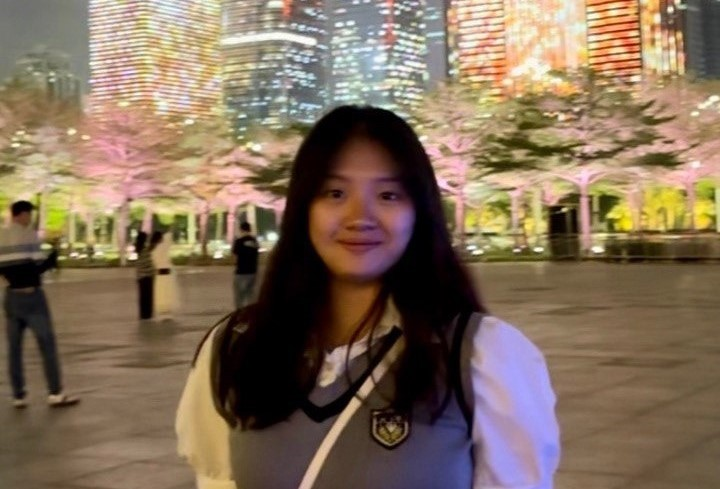
\includegraphics[width=\linewidth]{6275921855365889224.jpg}	%trimming relative to image size

%---------------------------------------------------------------------------------------
%	META CONTACT
%----------------------------------------------------------------------------------------
\vspace{26pt}
\cvsection{CONTACT} 
	
\icontext{MapMarker}{12}{30 Woodlands Dr 16, \\Forestville 11\#22\\Singapore 737769}{black}\\[8pt]
\icontext{MobilePhone}{12}{+65 98881351}{black}\\[8pt]
\begin{minipage}{\textwidth}
	\iconemail{Envelope}{12}{lawmingqi1818@gmail.com}{}{black}\\[8pt]
\end{minipage}
\begin{minipage}{\textwidth}
	\iconlinkedin{https://www.linkedin.com/in/law-ming-qi/}{}\\[6pt]
\end{minipage}


%---------------------------------------------------------------------------------------
%	META SKILLS
%----------------------------------------------------------------------------------------
\vspace{10pt}

\cvsection{TECHNICAL SKILL}

\cvskill{Python} {} {0.9} \\[-2pt]

\cvskill{C\#} {} {0.7} \\[-2pt]

\cvskill{Javascript} {Frontend, Backend} {0.8} \\[-2pt]

\cvskill{HTML \& CSS} {} {0.89} \\[-2pt]

\cvskill{Node.js \& Express.js} {Backend Development} {0.8} \\[-2pt]

\cvskill{MSSQL} {} {0.9} \\[-2pt]

\cvskill{Design Tools} {Figma, Adobe, Canva} {0.75} \\[-2pt]

\cvskill{GIT} {} {0.6} \\[-2pt]


%---------------------------------------------------------------------------------------
%	SOFT SKILLS
%----------------------------------------------------------------------------------------
\newpage
\cvsection{SOFT SKILLS}

\cvsoftskill{Courage to Take Risks}
\cvsoftskill{Assertiveness}
\cvsoftskill{Open-Mindedness}
\cvsoftskill{Goal-Oriented Mindset}
\cvsoftskill{Straightforward Communication}
\cvsoftskill{Self-Motivation}
\cvsoftskill{Resilience}






%---------------------------------------------------------------------------------------
% AWARDS 
%----------------------------------------------------------------------------------------
\vspace{1.6cm}
\cvsection{AWARDS}

\cvaward{2022}{
    - Edusave Scholarship Award from MOE \\ 
    - Eagles Award\\
    - Edusave Character Award
}
\cvaward{2019}{
	- Edusave Scholarship Award from \\Ministry of Education (MOE)
}


%---------------------------------------------------------------------------------------
%	CERTIFICATION
%----------------------------------------------------------------------------------------
\vspace{1.8cm}
\cvsection{CERTIFICATIONS}

\cvmetaevent
{PSM 1 - Professional Scrum Master 1}
{}
{}
{}
\cvmetaevent
{Google Project Management}
{}
{\cvlist{
	\item Project Execution: Running the Project
	\item Foundations of Project Management
	\item Project Planning: Putting It All Together
	\item Agile Project Management
	\item Project Initiation: Starting a Successful Project
}}
{}

\newpage
\mbox{} % hotfix to place qrcode on the bottom when there are not other elements
\vfill

\end{leftcolumn}
\begin{rightcolumn}
%---------------------------------------------------------------------------------------
%	TITLE  HEADER
%----------------------------------------------------------------------------------------
\fcolorbox{white}{royalpurple}{\begin{minipage}[c][3.5cm][c]{1\mpwidth}
	\begin {center}
		\HUGE{ \textbf{ \textcolor{white}{ \uppercase{ Law Ming Qi } } } } \\[-24pt]
		\textcolor{white}{ \rule{0.1\textwidth}{1.25pt}\\ }
		\large{ \textcolor{white} {Passionate Software Developer} } 
	\end {center}
\end{minipage}}

%---------------------------------------------------------------------------------------
%	PROFILE
%----------------------------------------------------------------------------------------
\vspace{30pt}
\cvsection{PROFILE}

\cvtext{
	I am a proactive IT student with a keen interest in the technology that shapes our daily lives and how it can be leveraged to drive innovation. 
	As an adaptable team player equipped with skills in backend, frontend development and database management, I thrive in fast-paced, deadline-driven environment
	and I am ready to apply both my academic and industry knowledge to tackle real-world challenges. 
	I remain committed to continuous learning and personal growth, always seeking to deepen my understanding of technology and its impact on society.

}

%---------------------------------------------------------------------------------------
%	EDUCATION
%----------------------------------------------------------------------------------------
\vspace{47pt}
\cvsection{EDUCATION}

\cvevent
{Apr 2023 - Present}
{Ngee Ann Polytechnic}
{Diploma in Information Technology}
{} 
{} 
{} 
{}

\cvevent
{2019 - 2022}
{Orchid Park Secondary School}
{GCE 'O' Level Certificate}
{Achieved \textbf{6 distinctions} in E Maths, A Maths, Chinese, Science (Bio/Chem), \\Principles of Accounts, Humanities (Social Studies/History)
\\\\L1R4: 9, L1R5: 11
}
{}
{} 
{} 
{} 
%---------------------------------------------------------------------------------------
%	WORK EXPERIENCE
%----------------------------------------------------------------------------------------
\vspace{25pt}
\cvsection{WORK EXPERIENCE}

\cvevent 
{Aug 2023 - Oct 2023} 
{Retail and E-commerce Associate} 
{Cold Storage - Singapore} 
{\cvlist{ \item Processed online orders and ensured timely delivery while assisting customers. }} 
{} 
{}
{}

\cvevent 
{Dec 2022 - Jan 2023} 
{Retail Assistant} 
{NTUC - Singapore} 
{\cvlist{ \item Provided customer assistance and maintained organized shelves. }} 
{}
{}
{}
\vfill\null


%---------------------------------------------------------------------------------------
%	CO-CURRICULAR ACTIVITIES 
%----------------------------------------------------------------------------------------
\newpage
\cvsection{CO-CURRICULAR ACTIVITIES (CCA)}

\cvevent
	{2023 - Present}
	{Ngee Ann Polytechnic}
	{Wushu}
	{\cvlist{
		\item \textbf{Captain}, Wushu School Team 
		\item \textbf{3rd Place}, NTU Invitational Wushu Championship 2024 Traditional Northern Fist.
		\item \textbf{3rd Place}, NTU Invitational Wushu Championship 2024 Group Routine, Fist.
		\item \textbf{2nd Place}, NTU Invitational Wushu Championship 2023 Traditional Other Fist.
		\item \textbf{1st Prize}, Youth Category Female, 1st International Nandao.
		\item \textbf{1st Prize}, Open Category Group Event Non-weapon.
	}}
	{}
	{}
	{}
	{}

\cvevent
	{2019 - 2022}
	{Orchid Park Secondary School}
	{Wushu}
	{\cvlist{
		\item \textbf{Captain}, Wushu School Team (2021 - 2022)
		\item Participated in the \textbf{National School Games (NSG)} in 2021 and 2022.
		\item Achieved \textbf{Top 10} in the 2022 NSG for 1st International Nandao Female \\category.
	}}
	{}
	{}
	{}


%---------------------------------------------------------------------------------------
%	ACADEMIC PROJECTS / COMPETITION PROJECTS 
%----------------------------------------------------------------------------------------
\vspace{30pt}
\cvsection{ACADEMIC PROJECTS / COMPETITION PROJECTS }\\[20pt]

\projects 
    {Competition: National AI Student Challenge 2024}
    {Track 2: Amazon Web Services (AWS)}
    {Feb 2024 - March 2024}
    { 
        \item Amazon SageMaker
        \item AWS Cloud Services
        \item LLaMA-2-7B-Chat (Large Language Model)
    }
    {}
	{
        \item Fine-tuned LLM by adjusting hyperparameters for optimal performance.
        \item Utilized AWS SageMaker for managing machine learning workflows, including model training and deployment.
        \item Prepared and augmented datasets to enhance model accuracy.
    }
	\newpage

\projects 
    {Module: Back-end Development}
    {Develop a community engagement website}
    {May 2024 - July 2024}
    { 
        \item HTML, CSS, Javascript, Bootstrap, Firebase, MSSQL, Node.js, Express.js
        \item Tools: Firebase Cloud Storage, RESTful APIs, CRUD operations
    }
    {}
	{
        \item Create a platform for users to register, log in, book facilities, register for events, and provide feedback, while staff manage and update website features.
        \item Implemented JWT-based authentication, Firebase integration for profile management, responsive design, real-time updates, and role-based access for staff.
    }


%---------------------------------------------------------------------------------------
%	ACTIVITIES
%----------------------------------------------------------------------------------------
\vspace{30pt}

\cvsection{ACTIVITIES}

\activities 
    {International Experience}
    {Overseas Immersion Programme to Shenzhen, China}
    {March 2024}
    {Participated in a 2-week immersion program in Shenzhen, China, focusing on industrial and cultural visits.}
	{}
    {}

\activities 
    {Leadership Dialogue}
    {Dialogue with Prime Minister Lawrence Wong}
    {2 July 2024}
    {Participated in a session where Prime Minister Wong addressed the impact of AI and technology on Singapore's economy, the importance of adapting to change, and fostering social solidarity.}
	{}
    {}    

% hotfixes to create fake-space to ensure the whole height is used
\mbox{}
\vfill
\mbox{}
\vfill
\mbox{}
\vfill
\mbox{}
\end{rightcolumn}
\end{paracol}
\end{document}

